\documentclass[]{book}

%These tell TeX which packages to use.
\usepackage{array,epsfig}
\usepackage{amsmath}
\usepackage{amsfonts}
\usepackage{amssymb}
\usepackage{amsxtra}
\usepackage{amsthm}
\usepackage{mathrsfs}
\usepackage{color}
\usepackage{graphicx}
\usepackage{float}

%Algorithm packages
\usepackage{algorithm}  
\usepackage{algpseudocode}  
\usepackage{amsmath}  
\renewcommand{\algorithmicrequire}{\textbf{Input:}}  % Use Input in the format of Algorithm  
\renewcommand{\algorithmicensure}{\textbf{Output:}} % Use Output in the format of Algorithm  
%Here I define some theorem styles and shortcut commands for symbols I use often
\theoremstyle{definition}
\newtheorem{defn}{Definition}
\newtheorem{thm}{Theorem}
\newtheorem{cor}{Corollary}
\newtheorem*{rmk}{Remark}
\newtheorem{lem}{Lemma}
\newtheorem*{joke}{Joke}
\newtheorem{ex}{Example}
\newtheorem*{soln}{Solution}
\newtheorem{prop}{Proposition}

\newcommand{\lra}{\longrightarrow}
\newcommand{\ra}{\rightarrow}
\newcommand{\surj}{\twoheadrightarrow}
\newcommand{\graph}{\mathrm{graph}}
\newcommand{\bb}[1]{\mathbb{#1}}
\newcommand{\Z}{\bb{Z}}
\newcommand{\Q}{\bb{Q}}
\newcommand{\R}{\bb{R}}
\newcommand{\C}{\bb{C}}
\newcommand{\N}{\bb{N}}
\newcommand{\M}{\mathbf{M}}
\newcommand{\m}{\mathbf{m}}
\newcommand{\MM}{\mathscr{M}}
\newcommand{\HH}{\mathscr{H}}
\newcommand{\Om}{\Omega}
\newcommand{\Ho}{\in\HH(\Om)}
\newcommand{\bd}{\partial}
\newcommand{\del}{\partial}
\newcommand{\bardel}{\overline\partial}
\newcommand{\textdf}[1]{\textbf{\textsf{#1}}\index{#1}}
\newcommand{\img}{\mathrm{img}}
\newcommand{\ip}[2]{\left\langle{#1},{#2}\right\rangle}
\newcommand{\inter}[1]{\mathrm{int}{#1}}
\newcommand{\exter}[1]{\mathrm{ext}{#1}}
\newcommand{\cl}[1]{\mathrm{cl}{#1}}
\newcommand{\ds}{\displaystyle}
\newcommand{\vol}{\mathrm{vol}}
\newcommand{\cnt}{\mathrm{ct}}
\newcommand{\osc}{\mathrm{osc}}
\newcommand{\LL}{\mathbf{L}}
\newcommand{\UU}{\mathbf{U}}
\newcommand{\support}{\mathrm{support}}
\newcommand{\AND}{\;\wedge\;}
\newcommand{\OR}{\;\vee\;}
\newcommand{\Oset}{\varnothing}
\newcommand{\st}{\ni}
\newcommand{\wh}{\widehat}

%Pagination stuff.
\setlength{\topmargin}{-.3 in}
\setlength{\oddsidemargin}{0in}
\setlength{\evensidemargin}{0in}
\setlength{\textheight}{9.in}
\setlength{\textwidth}{6.5in}
\pagestyle{empty}



\begin{document}


\begin{center}
{\Large COMP 540 \hspace{0.5cm} Homework 4}\\
\textbf{Peiguang Wang, Xinran Zhou}\\ %You should put your name here
Due: 3/05/2018 %You should write the date here.
\end{center}

\vspace{0.2 cm}


\subsection*{Part 4: Support vector machines for multi-class classification }

%% Problem 1
\begin{enumerate}
	\item It is possible that once in a while a dimension in the gradient check will not match exactly. What could such a discrepancy be caused by? Is it a reason for concern?
	\begin{soln}
		The discrepancy is caused by the non-differentiable part of the loss function. The loss function is non-differentiable in when $\theta^{(j)^{T}}x(i) - \theta^{y_i^{T}}x(i)+\Delta = 0$. \\
		It is not a reason for concern. The loss will not increase if gradient is computed this way. So it is not a reason for concern.  
	\end{soln}

    \item Loss history figure.
    \begin{soln}
    	The loss changes with iteration times. The loss history plot is shown in Figure \ref{fig:lossHistory}.
    	\begin{figure}[H]
    		\centering
    		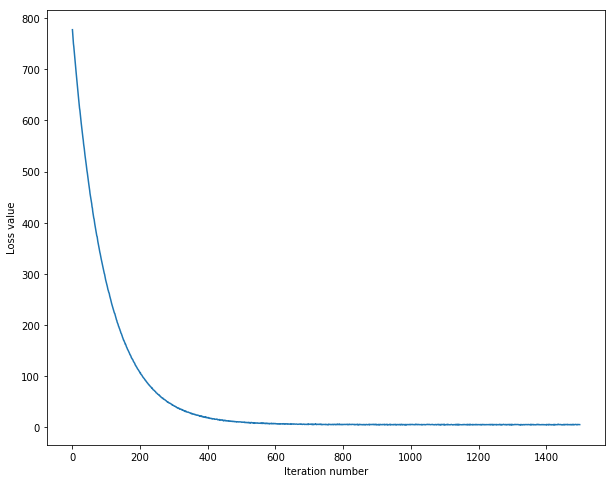
\includegraphics[width=8cm]{lossHistory.png}
    		\caption{Loss History}
    		\label{fig:lossHistory}
    	\end{figure}
    \end{soln}
    

    \item Search for the best svm model.
    \begin{soln}
    	Experiment with 4 learning rates and 4 regularization strengths. The result are:\\
    	\textit{lr 1.000000e-08 reg 1.000000e+04 train accuracy: 0.230592 val accuracy: 0.249000\\
    		lr 1.000000e-08 reg 5.000000e+04 train accuracy: 0.264000 val accuracy: 0.258000\\
    		lr 1.000000e-08 reg 1.000000e+05 train accuracy: 0.301898 val accuracy: 0.321000\\
    		lr 1.000000e-08 reg 5.000000e+05 train accuracy: 0.323796 val accuracy: 0.340000\\
    		lr 5.000000e-08 reg 1.000000e+04 train accuracy: 0.315531 val accuracy: 0.323000\\
    		lr 5.000000e-08 reg 5.000000e+04 train accuracy: 0.373837 val accuracy: 0.392000\\
    		lr 5.000000e-08 reg 1.000000e+05 train accuracy: 0.360265 val accuracy: 0.374000\\
    		lr 5.000000e-08 reg 5.000000e+05 train accuracy: 0.313184 val accuracy: 0.331000\\
    		lr 1.000000e-07 reg 1.000000e+04 train accuracy: 0.372735 val accuracy: 0.376000\\
    		lr 1.000000e-07 reg 5.000000e+04 train accuracy: 0.368714 val accuracy: 0.376000\\
    		lr 1.000000e-07 reg 1.000000e+05 train accuracy: 0.354429 val accuracy: 0.357000\\
    		lr 1.000000e-07 reg 5.000000e+05 train accuracy: 0.317000 val accuracy: 0.332000\\
    		lr 5.000000e-07 reg 1.000000e+04 train accuracy: 0.369204 val accuracy: 0.369000\\
    		lr 5.000000e-07 reg 5.000000e+04 train accuracy: 0.339816 val accuracy: 0.336000\\
    		lr 5.000000e-07 reg 1.000000e+05 train accuracy: 0.291224 val accuracy: 0.292000\\
    		lr 5.000000e-07 reg 5.000000e+05 train accuracy: 0.280633 val accuracy: 0.289000\\
    		lr 1.000000e-06 reg 1.000000e+04 train accuracy: 0.362796 val accuracy: 0.375000\\
    		lr 1.000000e-06 reg 5.000000e+04 train accuracy: 0.254204 val accuracy: 0.266000\\
    		lr 1.000000e-06 reg 1.000000e+05 train accuracy: 0.265082 val accuracy: 0.277000\\
    		lr 1.000000e-06 reg 5.000000e+05 train accuracy: 0.227735 val accuracy: 0.232000\\
    		best validation accuracy achieved during cross-validation: 0.392000}
    	
    	Visualized the results and the results are shown in Figure \ref{fig:train_acc}.
    	\begin{figure}[H]
    		\centering
    		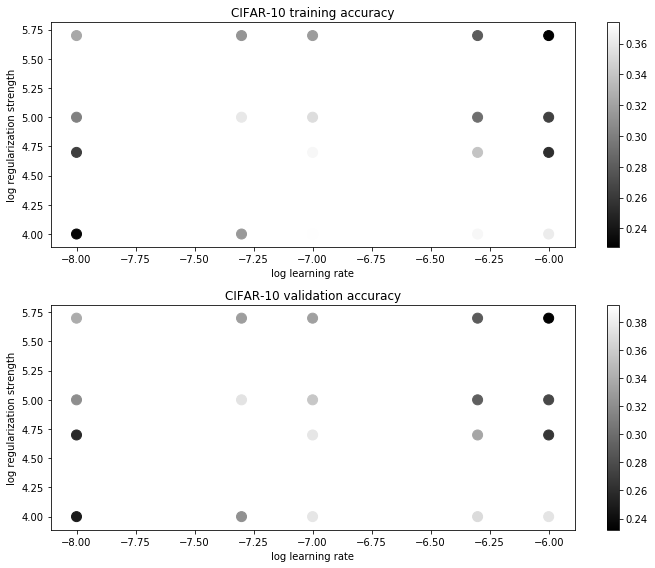
\includegraphics[width=8cm]{train_acc.png}
    		\caption{Visualized Results for Parameter Selection}
    		\label{fig:train_acc}
    	\end{figure}
    \end{soln}
    

	\item Evaluate the test set accuracy on the best svm learned.
	\begin{soln}
		After searching for the best values of learning rate and regularization. We obtain the best svm model. The results on the test set is: \textit{linear SVM on raw pixels final test set accuracy: 0.368300.}\\
		The accuracy is similar to the accuracy of validation set. Visualization of the results is shown in Figure \ref{fig:multiSVM}.
		
		\begin{figure}[H]
			\centering
			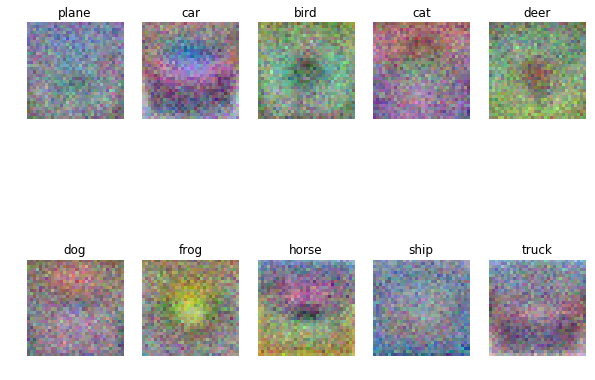
\includegraphics[width=8cm]{multiSVM_final.png}
			\caption{Visualized Results for Best SVM Multiclass Model}
			\label{fig:multiSVM}
		\end{figure}
	
	\end{soln}
	
	
	\item Comparing the performance of multi-class SVM and softmax regression. Which approach takes longer to train, which approach achieves higher performance? Compare the visualizations of the $\theta$ parameters learned by both methods - do you see any differences? Comment on hyper parameter selection for both methods.
	\begin{soln}
		\textbf{First compare the accuracy.}
		\begin{itemize}  
			\item Softmax on raw pixels final test set accuracy: 0.405100
			\item Linear SVM on raw pixels final test set accuracy: 0.368300.
		\end{itemize}
	    The accuracy on Softmax and SVM are almost the same level. Softmax is slightly higher than linear SVM method.
	    
	    \textbf{Then compare the visualization of these two methods.}\\
	    Figure \ref{fig:softmax} shows the results on softmax model.
	    \begin{figure}[H]
	    	\centering
	    	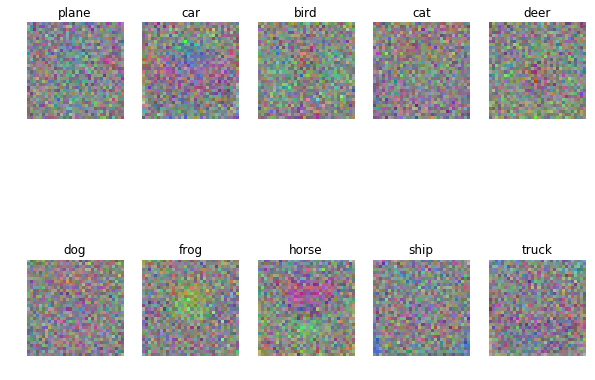
\includegraphics[width=8cm]{softmax_res.png}
	    	\caption{Visualized Results for Best Softmax Model}
	    	\label{fig:softmax}
	    \end{figure}
	    Figure \ref{fig:SVM} shows the results on SVM multiclass model.
	    \begin{figure}[H]
	    	\centering
	    	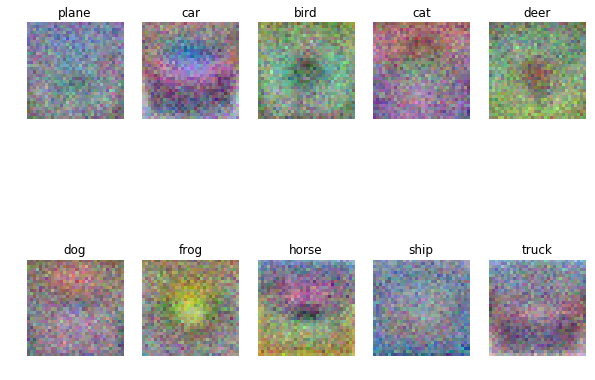
\includegraphics[width=8cm]{multiSVM_final.png}
	    	\caption{Visualized Results for Best SVM Multiclass Model}
	    	\label{fig:SVM}
	    \end{figure}
	    From the figure it seems the SVM model extracts a more "meaningful" features. Here "meaningful" means understandable for humans. The contour and edges are more clear in SVM model results.
	    
	    \textbf{Compare the time of these two methods.}
	    \begin{itemize}
	    	\item Softmax vectorized loss: 2.352202e+00 computed in 0.483000s
	    	\item Linear SVM Vectorized loss: 9.293820e+00 computed in 0.016000s
	    \end{itemize}
    	In terms of time cost. Softmax takes a much longer time to train. The reason is that SVM learns a sparse kernel.
    	
	    
		
	\end{soln}

\end{enumerate}



\end{document}


